\chapter{Rigid Bodies}
Rigid body's are defined by a particle that is the center of mass and a polygon. The weight distribution is equal in the complete rigid body.

To find points where forces have to be applied, a discrete version of the rigid body has to be found. This is done by simply walking over the bounding box and checking if the cell at that position is in the polygon. Let $P$ be the position that is checked.

It is also interesting to know to which points it is connected. This is done by checking the horizontal neighbours and vertical neighbours. Let this be $A_{P,1} .. A_{P,4}$. With this information all the boundary cells of a rigid object can be detected.

\section{User interaction}
It is possible to interact with the rigid object. If a rigid object is selected with the mouse, a spring force is created between the mouse and the particle at the center of the object.

\section{Boundaries}
With the information found it is easy to create boundaries for the liquid. For every adjacent cell the correct classification is determined. These classifications are described in chapter \ref{chap:BoundariesAndFixedObjects}.

\section{Body's to fluid}
Forces that are exerted on $A_{P,1} .. A_{P,4}$ (if they are liquid) are based on the velocity of cell $P$ in the object. The velocity  and the angular velocity of the object are both used to calculate the velocity of point $P$. This velocity is multiplied with a constant before applying it to the fluid. In figure \ref{fig:BodyToFluid} there is a scene where forces are applied from the body to the fluid.

\begin{figure}[htb!]
    \centering
    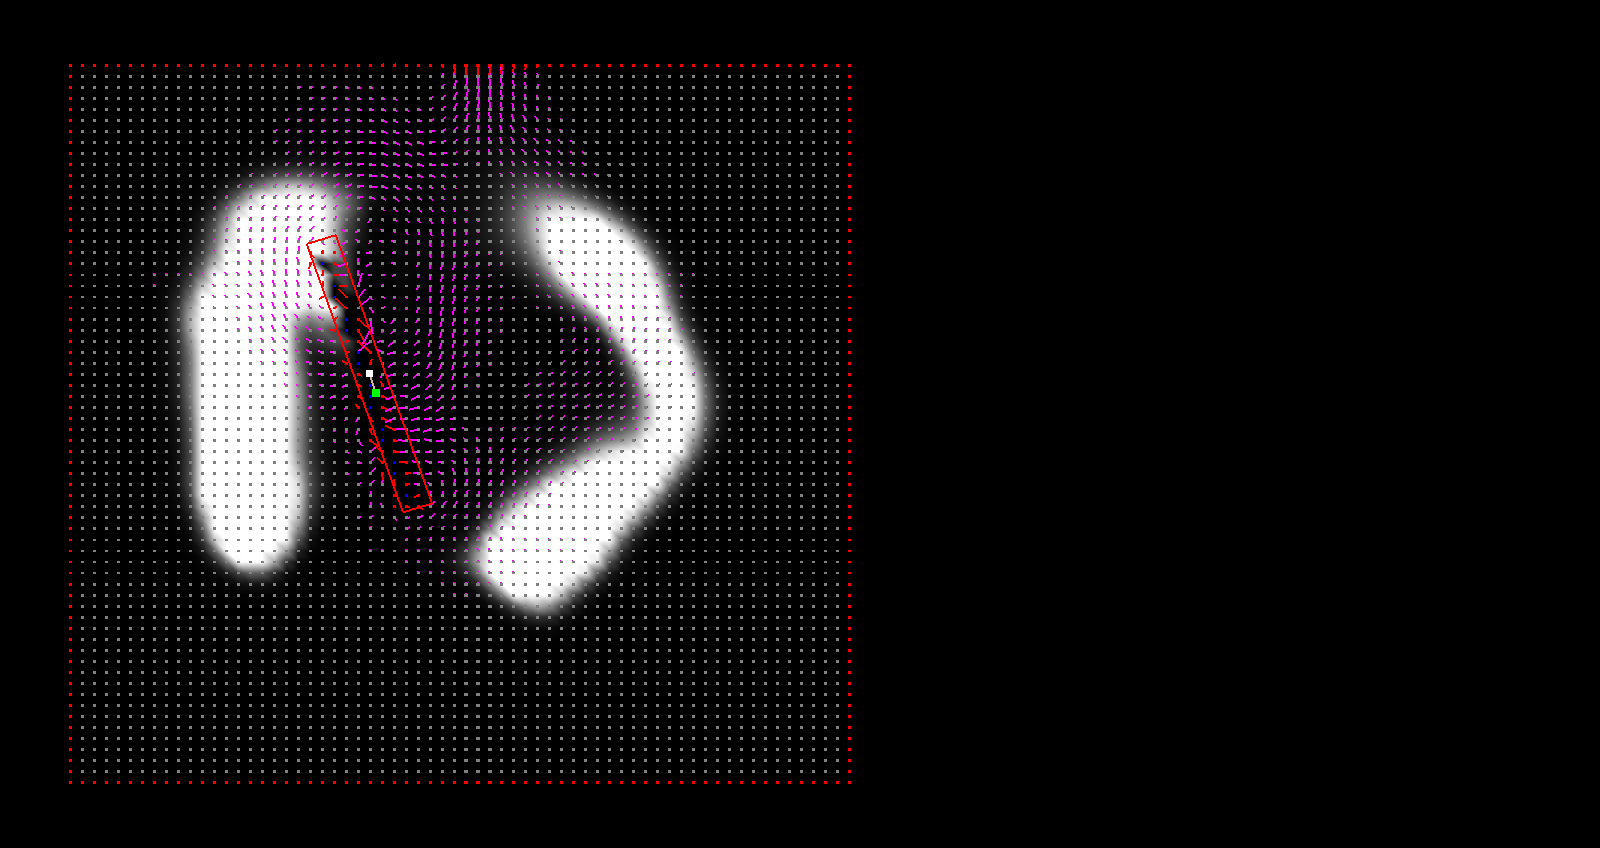
\includegraphics[width=0.6\textwidth]{images/BodyToFluid}
    \caption{A scene where forces from the body are applied to the fluid}
    \label{fig:BodyToFluid}
\end{figure}

\section{Fluid to Body's}
The force on point $P$ is calculated by the velocities in the adjacent cells $A_{P,1} .. A_{P,4}$ if there is liquid. The velocity is multiplied with its density at that point and a constant. The force on point $P$ is then transformed to linear force and rotation force on the object. In figure \ref{fig:FluidToBody} there is a scene where forces are applied from the fluid to the body. To create a more natural way of interacting with the rigid body a viscous drag is added, so it will stop when no force is being added.

\begin{figure}[htb!]
    \centering
    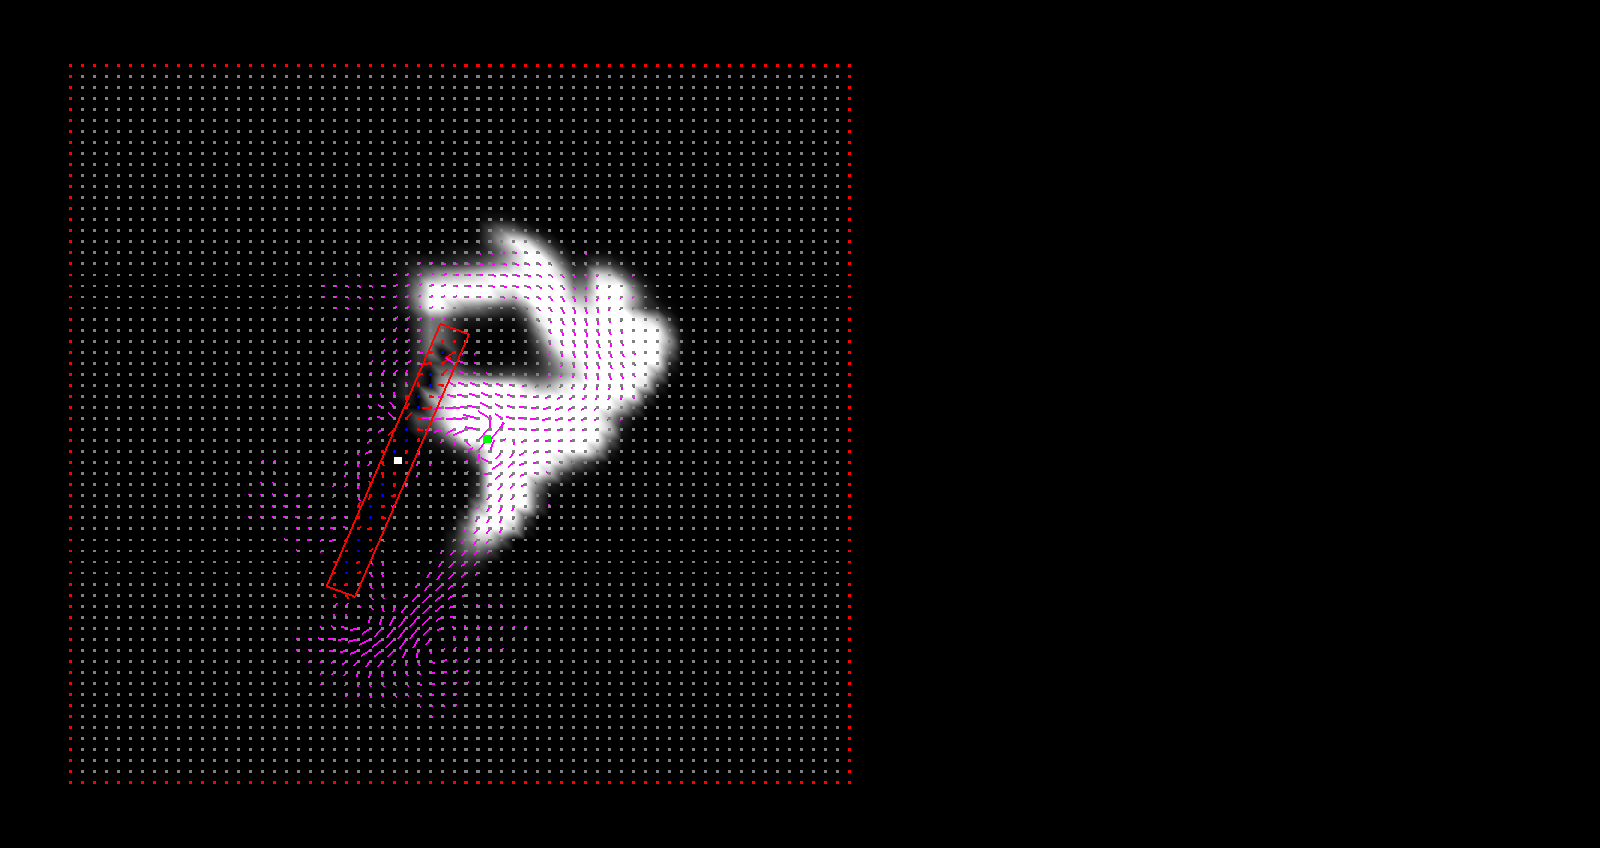
\includegraphics[width=0.6\textwidth]{images/FluidToBody}
    \caption{A scene where forces from the fluid are applied to the body}
    \label{fig:FluidToBody}
\end{figure}